\chapter{Introduction}

This part of the guide contains the information on using and developing \texttt{NekPy} 
Python wrappers for the \nek{} spectral/\textit{hp} element framework. 
\emph{As a disclaimer, these wrappings are experimental and incomplete.} 
You should not rely on their current structure and API remaining unchanged.

Currently, representative classes from the \texttt{LibUtilities}, \texttt{StdRegions},
\texttt{SpatialDomains}, \texttt{LocalRegions} and \texttt{MultiRegions} libraries 
have been wrapped in order to show the proof-of-concept.

\section{Features and functionality}

\texttt{NekPy} uses the \texttt{Boost.Python} library to provide a set of high-quality,
hand-written Python bindings for selected functions and classes in Nektar++. 

It is worth noting that Python (CPython, the standard Python implementation written in C, 
in particular) includes C API and that everything in Python is strictly speaking a C 
structure called \texttt{PyObject}. Hence, defining a new class, method etc. in Python 
is in reality creating a new \texttt{PyObject} structure.

Boost.Python is essentially a wrapper for Python C API which conveniently exports C++ 
classes and methods into \texttt{PyObjects}. At compilation time a dynamic library 
is created which is then imported to Python, as shown in Figure \ref{fig:boost_python}. 

\begin{figure}[h!]
	\centering
    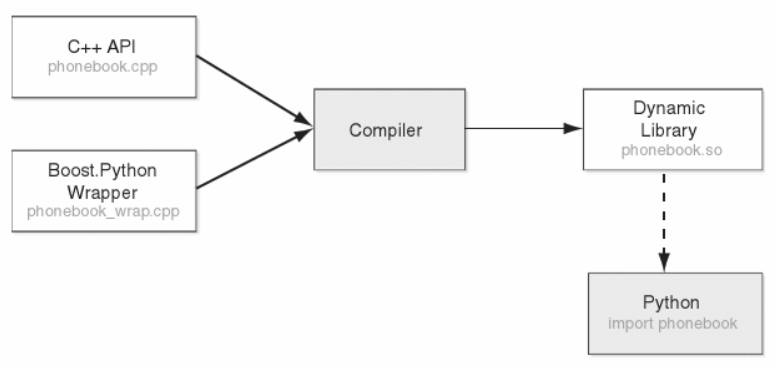
\includegraphics[width=0.9\textwidth]{img/boost_python}
    \caption{A schematic diagram of how C++ code is converted into Python with Boost.Python \cite{C++Api}}
    \label{fig:boost_python}
\end{figure}

A typical snippet could look something like:

\begin{lstlisting}[caption={NekPy sample snippet}, label={lst:nekpy_sample}, language=Python]
from NekPy.LibUtilities import PointsKey, PointsType, BasisKey, BasisType
from NekPy.StdRegions import StdQuadExp
import numpy as np
numModes = 8
numPts   = 9
ptsKey   = PointsKey(numPts, PointsType.GaussLobattoLegendre)
basisKey = BasisKey(BasisType.Modified_A, numModes, ptsKey)
quadExp  = StdQuadExp(basisKey, basisKey)
x, y     = quadExp.GetCoords()
fx       = np.sin(x) * np.cos(y)
proj     = quadExp.FwdTrans(fx)
\end{lstlisting}

\texttt{NekPy} uses the \texttt{Boost.NumPy} library, contained in Boost 1.63+, to
automatically convert C++ \texttt{Array<OneD, >} objects to and from the commonly-used
\texttt{numpy.ndarray} object, which makes the integration more seamless between Python
and C++.